\section{Bootstrap}
\subsection{Programmdownload}
\begin{itemize}
	\item Während der Entwicklung ist das Embedded System häufig über eine JTAG-Verbindung mit der      Entwicklungsumgebung verbunden 
	\item JTAG-Schnittstellen erfordern häufig (teure) Adapter, die für die Entwicklung akzeptabel,       im Betrieb aber zu teuer sind
	\item Für den Programmdownload im Betrieb steht häufig nur eine serielle Schnittstelle zur Verfügung
\end{itemize}

\subsection{Startvorgang (Booting)}
\begin{itemize}
	\item Das Starten eines Systems wird auch mit Booting bezeichnet
	\item Das Programm, welches beim Starten als erstes ausgeführt wird, heisst Bootloader oder Bootstrap loader 
	\item Der Bootloade rist für die ersten Initialisierungen verantwortlich und für das Starten des eigentlichen Programms (oft das Betriebssystem) 
\end{itemize}

\subsection{Mehrstufige Bootloader (multistage bootloader)}
\begin{itemize}
	\item Der Bootloader muss immer auf einem bootfähigen nicht flüchtigen Medium gespeichert sein
	\item Häufig wird der Bootloaderin mehreren Stufen aufgebaut, z.B. 
	\begin{itemize}
		\item erste Stufe initialisiert die Hardware und lädt ein bestimmtes Filesystem 
		\item die nächste Stufe ist als File in diesem Filesystem gespeichert und startet beispielsweise das Betriebssystem 
	\end{itemize}
	\item Vorteile: 
	\begin{itemize}
		\item die erste Stufe ist nur hardwarespezifisch, jedoch völlig unabhängig von Filesystem und Betriebssystem 
		\item  dadurch können diese Teile beliebig ausgetauscht und geändert werden 
		\item wenn die erste Stufe "nie" ändert, kann auch vermieden werden, dass sich das System durch eine fehlerbehaftete neue Version selbst abschiesst, d.h. dass dann das System nicht mehr ansprechbar wird
	\end{itemize}
\end{itemize}

\subsection{Sicherung des Programmdownloads}
\begin{itemize}
	\item Um die sichere Übertragung zu gewährleisten, wird diese meist mittels CRC (Cyclic Redundancy Check) gesichert
	\item Teilweise wird die Übertragung auch verschlüsselt, damit eine bösartige Änderung des Programms verhindert werden kann	
\end{itemize}

\begin{minipage}[c]{15cm}
	\subsection{Typische Memory Map}
	\begin{itemize}
		\item Der Bootloader liegt im nicht flüchtigen Bereich und wird nie geändert
		\item Das Programm ist meist im Flash EPROM und kann geändert werden oder das Programm wird von einer SD-Card ins RAM geladen
		\item Der Datenblock ist immer im RAM
		\item Weitere Speicherbereiche können für die Peripherie vorgesehen werden (Memory mapped I/O) oder bleiben ungenutzt
	\end{itemize}
	
	\subsection{Typischer Bootvorgang}
	\begin{enumerate}
		\item Beim Aufstarten wird immer zuerst das Bootloader-Programm gestartet
		\item In diesem Programm wird z.B. geprüft, ob über eine Kommunikationsverbindung ein neues Programm in den Programmbereich geschrieben werden soll 
		\item Wenn ein neues Programm geschrieben werden soll, dann wird dieses mit Hilfe eines definierten Protokolls übertragen und geschrieben 
		\item Wenn das Programm fertig übertragen wurde oder das bestehende ausgeführt werden soll, wird mit der Ausführung an dieser Stelle fortgefahren
	\end{enumerate}
\end{minipage}
\hspace*{0.5cm}
\begin{minipage}[c]{3.2cm}
	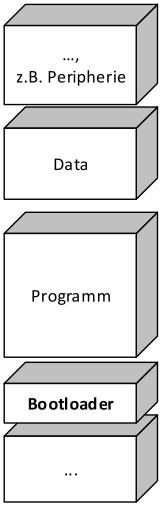
\includegraphics[width=1\textwidth]{images/Bootstrap/Bootstrap}
\end{minipage}

